\documentclass[a4paper]{jpconf}
\usepackage{graphicx}
\usepackage{caption}
\begin{document}
\title{Estimation of jet-faked muon background in W-boson scattering at $\sqrt{s} = 13 \ TeV$ with the ATLAS detector}
\author{Lucas Michael Henry McConnell \\ Supervised by: Dr A. Hamilton and Dr S. Yacoob}
\address{Department of Physics, University of Cape Town, South Afirca}
\ead{lucas.mcconnell@cern.ch}
\begin{abstract}
$ W^{\pm}W^{\pm} \longrightarrow W^{\pm}W^{\pm}$ is a rare Standard Model process which can be used to investigate the spontaneous symmetry breaking present in the Standard Model. Previous analysis, using $\sqrt{s} = 8$ TeV proton-proton collision data recorded by the ATLAS detector at the Large Hadron Collider, of events with two reconstructed same sign leptons ($e^{\pm}e^{\pm}$,$e^{\pm}\mu^{\pm}$, and $\mu^{\pm}\mu^{\pm}$) and two jets were analysed and $W^{\pm}W^{\pm}jj$ production cross sections were measured. First evidence for $W^{\pm}W^{\pm}jj$ production was observed to a significance of $4.5 \ \sigma$. Starting in 2015, analysis is underway to attempt to increase the significance for the measurements using $\sqrt{s} = 13$ TeV proton-proton collision data recorded by the ATLAS detector at the Large Hadron Collider. Since the process is very rare, it is dominated by various backgrounds, one of which is $t\bar{t}$ decay. In this presentation we discuss estimating the fake muon background coming from $t\bar{t}$ decay using Monte Carlo simulations.
\end{abstract}
\section{The Standard Model of Particle Physics}
The Standard Model \cite{stdmd1,stdmd2,stdmd3,stdmd4} of particle physics was developed in the latter half of the twentieth century. It describes how matter is compromised of point-like, basic building blocks called fundamental particles, and interacts via four fundamental forces. The Standard Model has successfully been tested many times and is widely regarded as the most accurate and stable \cite{stdmd_fit} model of particle physics.

The Standard Model classifies the fundamental particles that make up matter into either lepton or quarks. Both leptons and quarks comes in three so-called generations, with the members of the first generation being the lightest and most stable, while those of the third generation are the heaviest and least stable. In ascending order of generation the leptons are: the electron and electron neutrino, the muon and muon neutrino, and the tau and tau neutrino. These particles posses half-integer spin and are known collectively as \emph{fermions}.

The Standard Model describes three of the four fundamental interactions in nature. In increasing order of strength, these are the weak, electromagnetic, and strong forces. According to the Standard Model, the strong, weak, and electromagnetic forces result from the exchange of force-carrier particles. These force carriers posses integer spins and are collectively called \emph{bosons}. Specific bosons are said to mediate a particular force. The strong force is mediated by the gluon, the electromagnetic by the photon, and the weak by the W and Z bosons.

A deficiency of the Standard Model is that it does not describe the gravitational interaction. Theories that seek to expand upon the Standard Model in order to incorporate gravity are said to be "beyond" the Standard Model.
\section{The ATLAS Detector}
Some of the experimental confirmation of the Standard Model has come from the European Organization for Nuclear Research (CERN) in Switzerland. In particular CERN is home to the largest and most powerful particle accelerator in the world: the Large Hadron Collider (LHC) \cite{lhc}. The ATLAS (A Toroidal LHC Apparatus) detector \cite{atlas} is one of the seven particle detectors at the LHC and is one of two general purpose detectors designed to take advantage of the unprecedented energy available at the LHC and investigate physical phenomena that involve high mass particles that were not previously observable at earlier low-energy accelerators. In particular the ATLAS experiment has been involved in the search for the Higgs boson \cite{atlas_higgs}, extra dimensions and dark matter particles \cite{atlas_dm_ed}. ATLAS is 46 metres long, 25 metres in diameter and has a mass of about 7000 tonnes.
\section{W-Boson Scattering}
The scattering of \emph{W-bosons} can be a useful process in the probing of electroweak symmetry breaking. Without a Higgs boson the longitudinally polarised amplitude of W-boson scattering violates unitarity when the \emph{WW} centre-of-mass energy exceeds approximately 1 TeV \cite{violation1,violation2,violation3}. With the discovery of the 125 GeV Higgs boson \cite{atlas_higgs,cms_higgs} , the high energy value of the cross-section again becomes unitarised within the Standard Model, giving insight as to whether it is the Standard Model Higgs boson.

The \emph{W-boson} scattering can be either opposite-sign $W^{\pm}W^{\mp}$ or same-sign $W^{\pm}W^{\pm}$. The case of opposite-sign scattering is dominated by background contributions from \emph{Quantum Chromodynamics (QCD)}. This is however not the case for same-sign scattering and thus it is expected to more sensitive to the quartic coupling. Considering the leptonic decays of the \emph{W-boson}, the distinctive experimental signature for this study is then two same-sign leptons ($e^{\pm}e^{\pm},e^{\pm}\mu^{\pm},\mu^{\pm}\mu^{\pm}$), along with two jets, and missing transverse energy from neutrinos. This is graphically represented in Fig (\ref{signal_process}).
\begin{figure}[!tbp]
\centering
\begin{minipage}[b]{.4\textwidth}
  \centering
  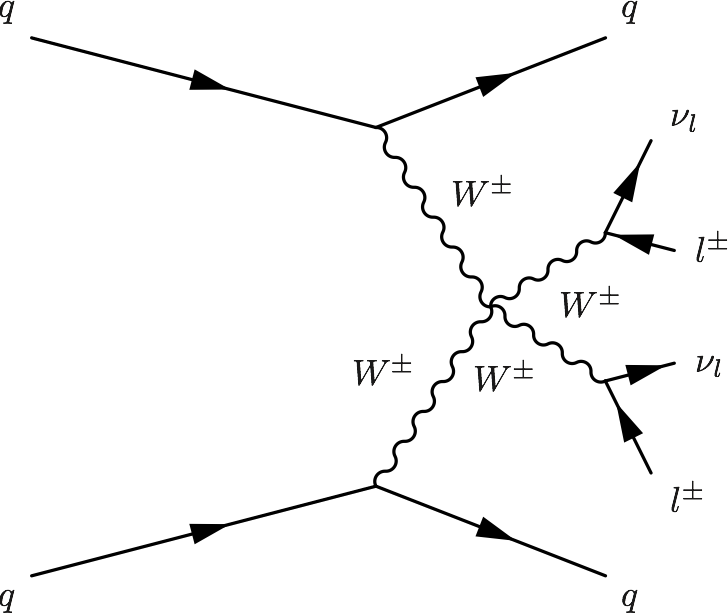
\includegraphics[width=\textwidth]{signal.png}
  \captionof{figure}{Feynman diagram showing the scattering of two same-sign \emph{W-bosons} which subsequently decay leptonically.}
  \label{signal_process}
\end{minipage}
\hfill
\begin{minipage}[b]{.55\textwidth}
  \centering
  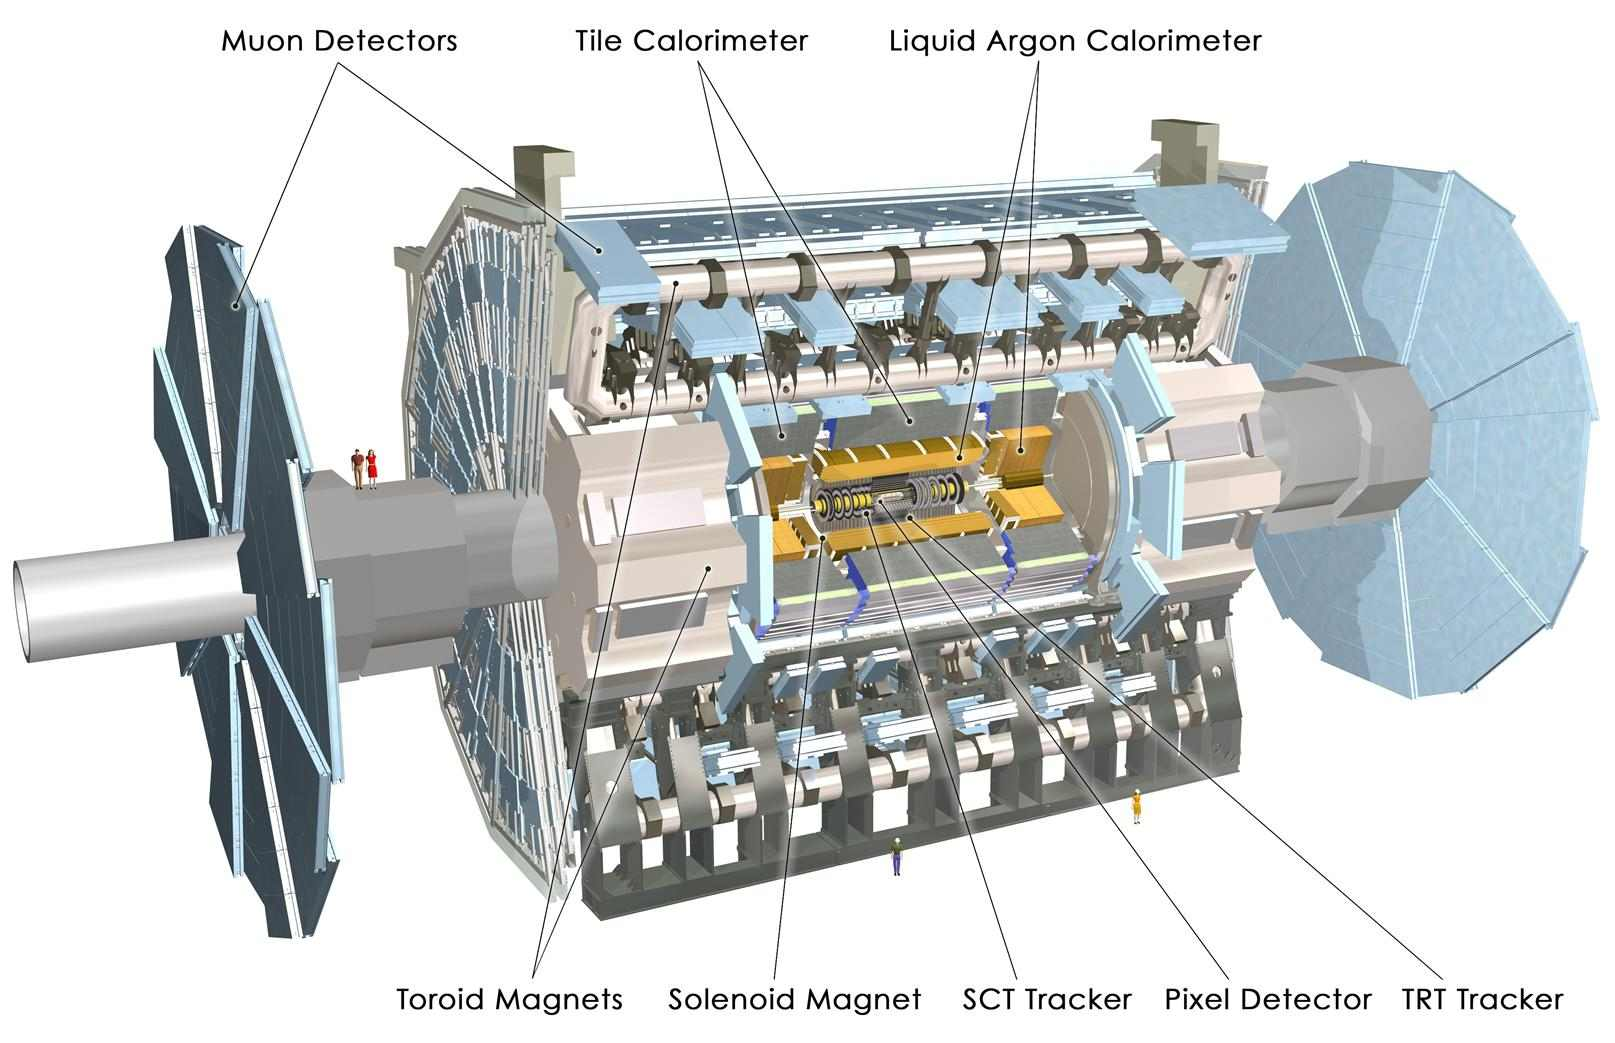
\includegraphics[width=1\textwidth]{atlas.png}
  \captionof{figure}{Cut-away view of the ATLAS detector showing its various components. \cite{atlas_diagram}}
  \label{atlas}
\end{minipage}
\end{figure}

First evidence for same-sign \emph{WW} (\emph{ssWW}) scattering using $\sqrt{s} = 8 \ TeV$ proton-proton collision data was found with a significance of $4.5 \ \sigma$ by ATLAS \cite{atlas_result}, while a similar analysis by the CMS experiment \cite{cms_result} found a significance of $2.0 \ \sigma$. These proceedings report on some of the work to increase the significance for the measurement using $\sqrt{s} = 13 \ TeV$ proton-proton collision data recorded by the ATLAS detector.
\section{Fake Lepton Background}
Leptons coming from a \emph{W-boson} are said to be prompt, while those those coming from the decay of a hadron are said to be non-prompt.  Non-prompt leptons contribute to background in events selected for \emph{ssWW} measurement. This background is subsequently referred to in this note as the \emph{fake lepton background}. The dominant contribution to the fake lepton backgrounds comes from the process $t\bar{t} \longrightarrow WbWb \longrightarrow \ell\nu bb qq$.

The degree to which leptons are \emph{isolated} can be used to reduce the fake lepton background. Isolation is a measure of the number of particles produced in a cone in $\eta - \phi$ space, defined by $\Delta R = \sqrt{(\Delta\eta)^{2} + (\Delta\phi)^{2}}$,with $\eta$ being pseudorapidity and $\phi$ being the azimuthal angle, around the detector signature corresponding to the reconstructed lepton. ``$p_{T}cone20$'' is the sum of the transverse momenta of all tracks within a cone of $\Delta R = 0.20$, while ``$e_{T}cone20$'' is the sum of the transverse energy within a $\Delta R = 0.20$ centred on the lepton's deposit in the calorimeter. Since hadrons are often produced in collimated flows, called jets, fake leptons are less likely to be isolated than prompt leptons. The primary goal of this work is to optimise the event selection criteria related to the lepton isolation to reduce the \emph{fake lepton background}.
\section{Conclusion}
The plots shown in Fig (\ref{money_plot}). display the isolation variables for muons with three different origins. The $t\bar{t}$ sample is produced using the \emph{PowHeg-Box} event generator \cite{powheg}, while \emph{ssWW} sample is produced by the \emph{Sherpa} event generator \cite{sherpa}. Using a $t\bar{t}$ sample as a background, reconstructed muons were matched to truth muons using the standard ATLAS Mone Carlo (MC) truth classifier tool. It was found that the majority of the background muons come from either \emph{W-bosons} ($63\%$) or \emph{b-mesons} ($12\%$), representing a prompt and non-prompt background respectively.

These backgrounds are plotted with the \emph{ssWW} sample. Note that the muons from the \emph{ssWW} and the prompt background muons are similarly isolated since both originate from \emph{W-bosons}. The muons coming from \emph{b-mesons} are less isolated, indicative of the muon having originated from a jet. A large fraction, $34\%$, of the reconstructed muons are unable to be truth-matched using the MC classifier tool. \emph{See the SAIP 2016 poster by Xolisile Thusini for the efforts to the classify these leptons coming from an unknown origin.}
\begin{figure}[h]
\centering
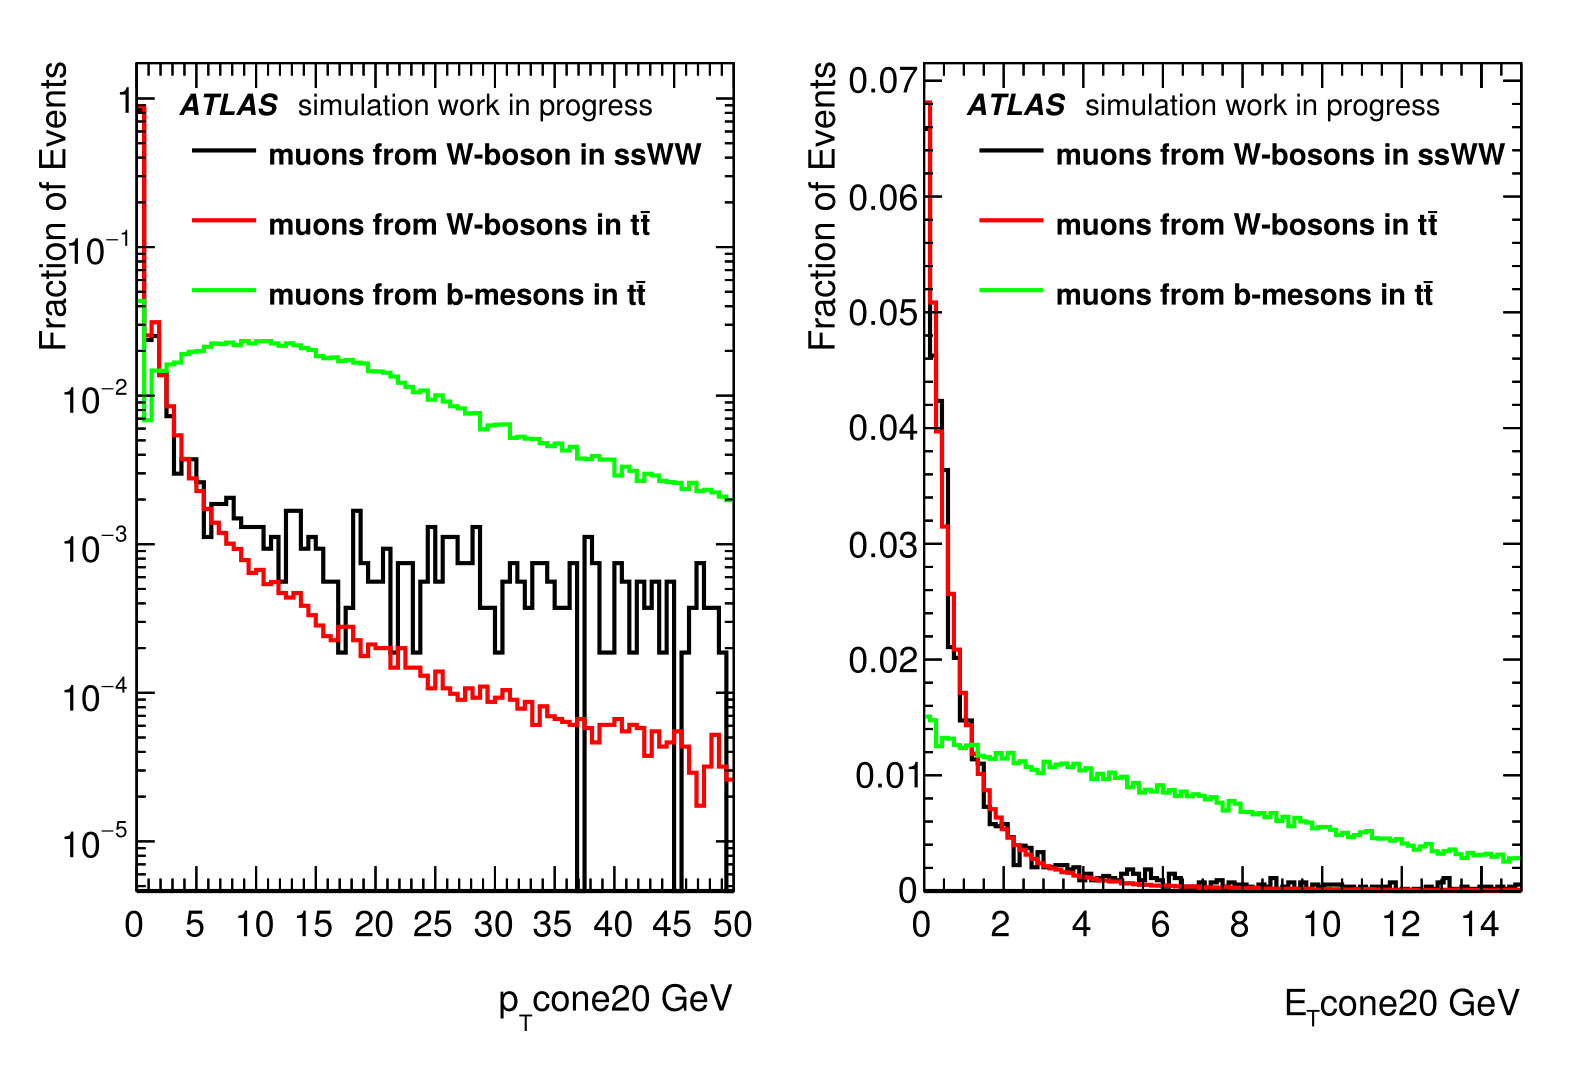
\includegraphics[width=0.8\textwidth]{iso_vars.png}
\caption{Simulation plots of the isolation variables for reconstructed muons with three different origins.}
\label{money_plot}
\end{figure}
\section{Future Studies}
Cuts motivated by the plots in Fig \ref{money_plot}. suggest how the signal-to-background ratio may be optimised in analysis using experimental data.
\newpage
\section*{References}
\begin{thebibliography}{9}
\bibitem{stdmd1} S. L. Glashow, \textit{Nucl. Phys.} \textbf{22} (1961) 579
\bibitem{stdmd2} S. Weinberg, \textit{Phys. Rev. Lett.} \textbf{19} (1967) 1264
\bibitem{stdmd3} A. Salam, \textit{Conf. Proc. C} \textbf{680519} (1968) 367
\bibitem{stdmd4} G. S. Guralnik and C. R. Hagen and T. W. B. Kibble, \textit{Phys. Rev. Lett.} \textbf{13} (1964) 20
\bibitem{stdmd_fit}M.~Baak and R.~Kogler, arXiv:1306.0571 [hep-ph].
\bibitem{atlas_diagram} ATLAS Collaboration, arXiv:1305.4551 [hep-ex].
\bibitem{lhc} L. Evans and P. Bryant (editors), \textit{JINST} \textbf{3} (2008) S08001
\bibitem{atlas} ATLAS Collaboration, \textit{JINST} \textbf{3} (2008) S08003
\bibitem{atlas_higgs} ATLAS Collaboration, \textit{Phys. Lett.} \textbf{B716} (2012) 1
\bibitem{atlas_dm_ed} ATLAS Collaboration, \textit{Phys. Lett.} {\bf B710} (2012) 538
\bibitem{violation1} M.~ J.~ G.~ Veltman, \textit{itActa Phys. Polon} \textbf{B8} (1977) 475
\bibitem{violation2} B.~ W.~ Lee and C.~ Quigg and H.~ B.~ Thacker, \textit{Phys. Rev. Lett.} \textbf{38} (1977) 883
\bibitem{violation3} B.~ W.~ Lee and C.~ Quigg and H.~ B.~ Thacker, \textit{Phys. Rev. Lett.} \textbf{D16} (1977) 1519
\bibitem{cms_higgs} CMS Collaboration, \textit{Phys. Lett.} \textbf{B716} (2012) 30
\bibitem{atlas_result} ATLAS Collaboration, \textit{Phys. Rev. Lett.} \textbf{113} (2014), 141803
\bibitem{cms_result} CMS Collaboration, \textit{Phys. Rev. Lett.} \textbf{114}, 051801
\bibitem{powheg} S. Frixione, P. Nason, and C. Oleari, \textit{JHEP} \textbf{0711} (2007) 070
\bibitem{sherpa} T. Gleisberg, S. Hoeche, F. Krauss, M. Schonhrtt, S. Schumann, et al., \textit{JHEP} \textbf{0902} (2009) 007
\end{thebibliography}
\end{document}